\begin{frame}{Overordnede kategorier af jagthunde}

\vspace{1em}

\begin{columns}[c] % c = center vertically

\column{0.05\textwidth} % Venstre margin

\column{0.7\textwidth} % Midten: Bullets

\small

\raggedright

\begin{itemize}

\itemsep0.6em % Justér afstand mellem bullets

\item \textbf{Stående} (f.eks. Irsk Setter)
\item \textbf{Stødende} (f.eks. Cocker Spaniel)
\item \textbf{Apporterende} (f.eks. Labrador, Golden Retriever)
\item \textbf{Gravsøgende} (f.eks. Gravhund)
\item \textbf{Støvende (drivende)} (f.eks. Beagle)
\item \textbf{Schweisshunde} (f.eks. Blodhund)

\end{itemize}

\column{0.25\textwidth} % Højre: Ikon

\centering

\vspace{0pt}

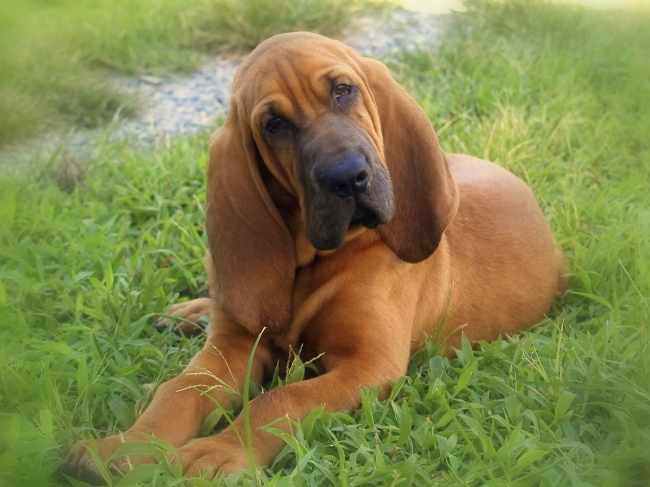
\includegraphics[width=0.9\linewidth]{Billeder/Jagthunde/schweisshunde/blodhund.jpg} % Ændret ikon til at passe med 'Hunde'

\end{columns}

\end{frame}